
Le protocole LoRaWAN a brièvement été introduit dans l'état de l'art de ce document en \cref{sec_stateOfTheArtLoRa}, mais il est particulièrement important de comprendre le fonctionnement de ce protocole afin d'en tirer la meilleure implémentation possible. LoRaWAN est développé et maintenu par la LoRa Alliance\footnote{\url{https://www.lora-alliance.org/}} dont les principaux membres du comité sont des grands noms du domaine\footnote{\url{https://www.lora-alliance.org/board-officers}}. On retrouve bien sûr Semtech qui fournit la technologie, mais également des grands noms de la télécommunication, tels que Orange ou Bouygues Telecom. 

Le protocole LoRaWAN est un protocole définissant la sous-couche \textit{Medium Access Control} (MAC), la couche liaison du modèle OSI\footnote{\url{https://en.wikipedia.org/wiki/OSI_model}}, ainsi que la couche 3 (réseau). Le protocole LoRaWAN peut être implémenté sur une modulation LoRa ou FSK \cite{HomeTheT94:online}.

\begin{figure}[ht!]
    \centering
    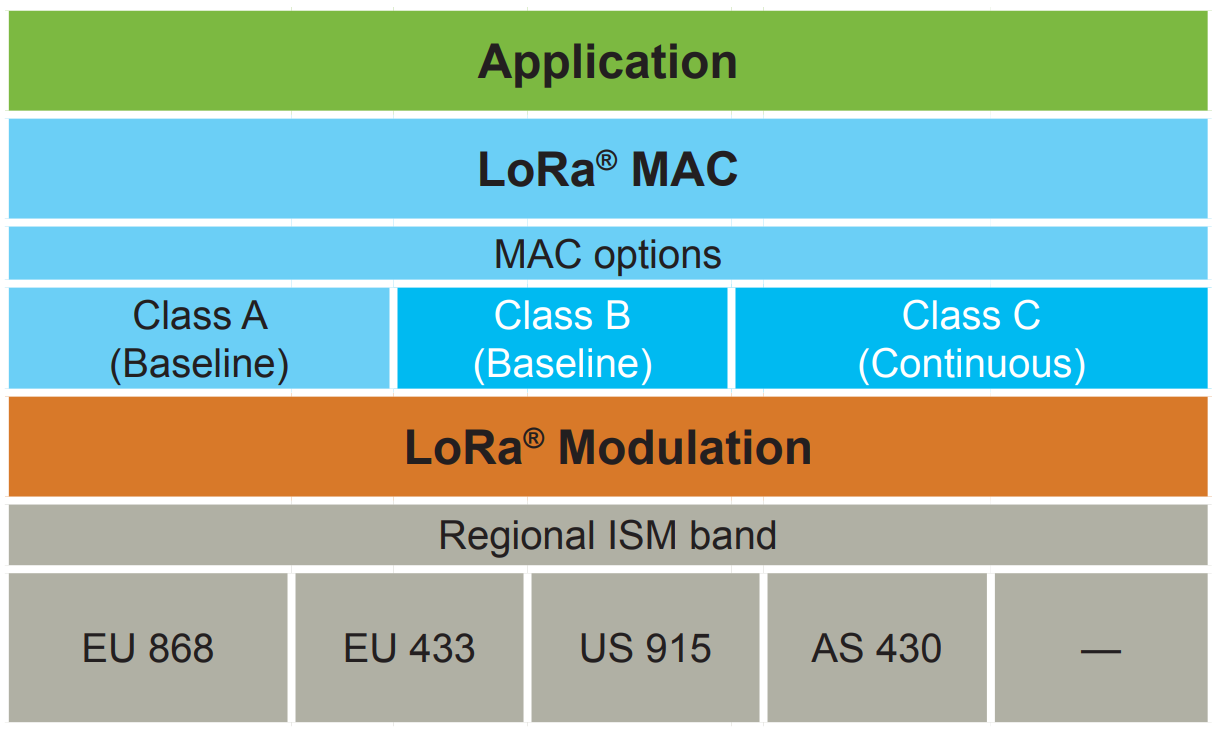
\includegraphics[width=0.65\textwidth]{Figures/Protocols/LoRaWAN/lorawan_and_lora_stack.PNG}
    \caption{Architecture du protocole LoRaWAN}
    \label{fig-lorawan_and_lora_stack}
\end{figure}

L'architecture complète du protocole LoRaWAN est visible en \cref{fig-lorawan_and_lora_stack} à sa base se trouve la couche LoRa comportant différentes fréquences en fonction de la région. Vient ensuite le concept de classe pour les périphériques. Ces classes définissent le comportement des périphériques vis-à-vis du réseau et seront développées plus en détail en \cref{sec-protocols_lorawan_classes}. Vient ensuite toute la partie LoRa MAC avec l'implémentation du protocole LoRaWAN. Toute la formation du paquet avec ses entêtes et ses données se trouve dans ce dernier élément.



\subsection{Classes des périphériques}
\label{sec-protocols_lorawan_classes}

LoRaWAN est un protocole bidirectionnel, assorti de quelques conditions. Il existe trois classes de périphériques. LoRaWAN définit ces trois classes \cite{LoRaWANd15:online} comme ceci : 
\begin{enumerate}
    \item Classe A (\textit{baseline}) : lorsqu'un périphérique envoi un message \textit{uplink}, il se met en écoute durant un laps de temps défini sur deux fenêtres de réception. La séquence de réception pour cette classe est visible sur la \cref{fig-class_a_rx}. C'est la classe qui consomme le moins d'énergie, car l'écoute ne se produit qu'après l'envoi d'un paquet. Quand le périphérique n'est pas ni en émission, ni en écoute de réponse, il peut être placé en veille profonde pour économiser un maximum d'énergie.
    %Dans l'option 1, la \textit{gateway} n'envoi pas de \textit{downlink} après l'\textit{uplink}. A l'inverse dans l'option 2 ou 3, une donnée est envoyée et reçue sur le périphérique. 
    
\begin{figure}[ht!]
    \centering
    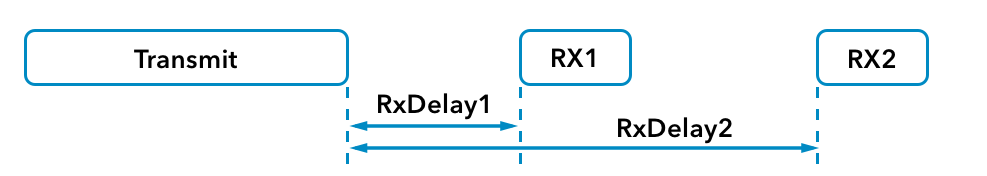
\includegraphics[width=0.9\textwidth]{Figures/Protocols/LoRaWAN/class_a_rx.png}
    \caption{Réception en tant que périphérique de type classe A}
    \label{fig-class_a_rx}
\end{figure}

    
    \item Classe B (\textit{beacon}) : Cette classe est identique à la classe A, mais offre la possibilité supplémentaire de programmer des fenêtres d'écoutes régulières que le périphérique doit écouter. La synchronisation temporelle de ces fenêtres s'effectue à l'aide de \textit{beacons} envoyés par la \textit{gateway} \cite{HomeTheT94:online,}. L'implémentation de cette classe a été finalisée dans la spécification 1.1 de LoRaWAN (cf. \cref{sec-protocols_lorawan_spec_1_1}). La \cref{fig-class_b_rx} illustre cette fenêtre de synchronisation.
   
\begin{figure}[ht!]
    \centering
    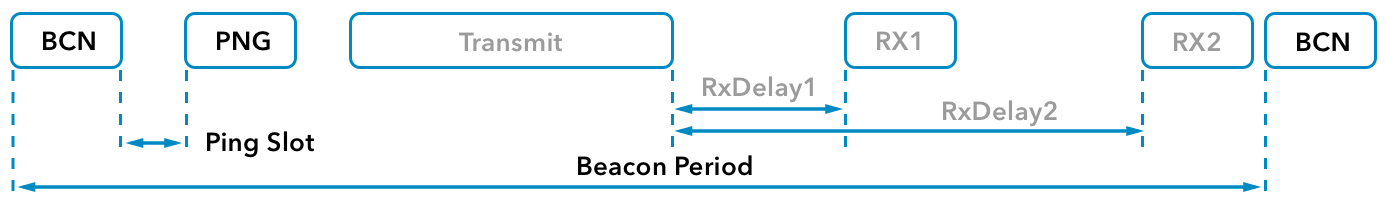
\includegraphics[width=0.9\textwidth]{Figures/Protocols/LoRaWAN/class_b_rx.png}
    \caption{Réception en tant que périphérique de type classe B}
    \label{fig-class_b_rx}
\end{figure} 

    
    \item Classe C (\textit{continuous}) : Cette classe est en écoute permanente sur une des fenêtres de réception, excepté lorsqu'un message est envoyé. On peut voir l'effet sur la \cref{fig-class_c_rx}. Cela a pour avantage de réduire la latence des communications \textit{downlink}, le périphérique n'ayant plus besoin d'un \textit{uplink} pour recevoir le message. En contrepartie, le périphérique consomme en permanence de l'énergie pour recevoir ces données. Cette option est uniquement envisageable si l'autonomie du périphérique ne constitue pas un problème.
    
\begin{figure}[ht!]
    \centering
    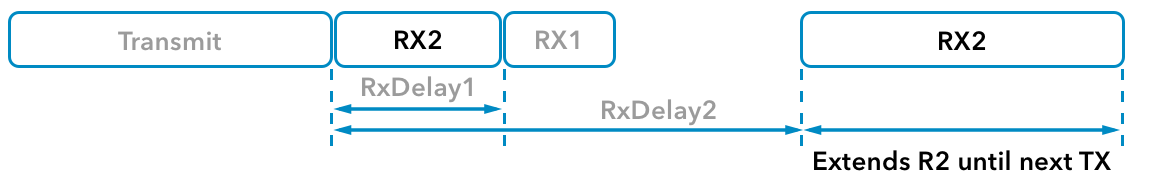
\includegraphics[width=0.9\textwidth]{Figures/Protocols/LoRaWAN/class_c_rx.png}
    \caption{Réception en tant que périphérique de type classe C}
    \label{fig-class_c_rx}
\end{figure}
\end{enumerate}



\subsection{Architecture d'un réseau LoRaWAN}
\label{sec-protocols_lorawan_architecture}
%https://www.tuv.com/media/corporate/products_1/electronic_components_and_lasers/TUeV_Rheinland_Overview_LoRa_and_LoRaWANtmp.pdf


\begin{figure}[ht!]
    \centering
    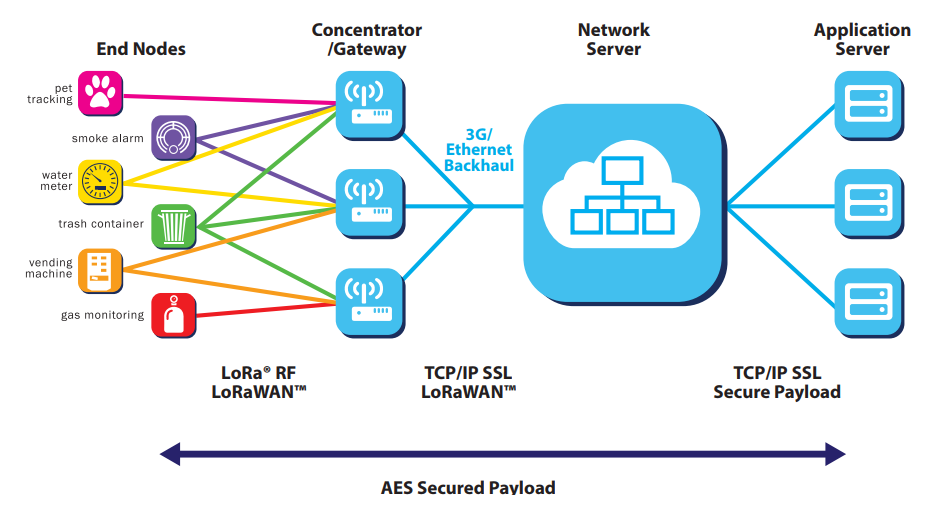
\includegraphics[width=0.95\textwidth]{Figures/Protocols/LoRaWAN/lorawan_archtecture.png}
    \caption{Architecture d'un réseau LoRaWAN}
    \label{fig-lorawan_archtecture}
\end{figure}

La \cref{fig-lorawan_archtecture} illustre l'architecture d'un réseau LoRaWAN avec ses divers composants. Les différents éléments de ce diagramme seront examinés plus en détail dans les sous-sections suivantes.


\subsubsection{\textit{End nodes}}
Les \textit{end nodes} sont les périphériques qui sont connectés au réseau. Ceux-ci sont tous équipés d'un module LoRa de la catégorie \textit{transceivers.}\footnote{\url{https://www.semtech.com/products/wireless-rf/lora-transceivers}}. La carte développée dans le cadre de ce projet entre dans cette catégorie. Un \textit{end node} LoRaWAN est souvent pourvu d'un dispositif basse consommation qui effectue une acquisition et envoie périodiquement des données à une application à travers le réseau. 



\subsubsection{\textit{Gateways}}

Les concentrateurs sont le pont entre un réseau LoRa et un réseau TCP/IP. Ceux-ci sont tous équipés d'un ou plusieurs modules LoRa de type concentrateur\footnote{\url{https://www.semtech.com/products/wireless-rf/lora-gateways}}. Les \textit{gateways} peuvent être achetées directement chez certains fabricants, mais il est également possible de créer sa propre \textit{gateway} à l'aide d'un Raspberry Pi et d'un concentrateur LoRa connecté via une communication série\footnote{\url{https://github.com/ttn-zh/ic880a-gateway/wiki}}. L'une des \textit{gateway} les plus utilisées est la Multitech Conduit, visible sur la \cref{fig-multitech_conduit}.

Le rôle de la \textit{gateway} consiste à démoduler les signaux reçus dans un \textit{buffer} afin de repérer la présence de trames LoRa. Tous les paquets sont transférés au \textit{Network Server}, quand bien même ils ne sont pas du réseau LoRaWAN auquel appartient la \textit{gateway}. Des métadonnées sont également ajoutées au paquet, tel que le \textit{Receive Signal Strength Indicator} (RSSI), \textit{Signal To Noise Ratio} (SNR), le canal de fréquence utilisé, le \textit{data rate}, ainsi que le \textit{Time of Arrival} (ToA). Les \textit{gateways} n'ont aucune information concernant les périphériques connectés au réseau. Elles ne font que transférer les paquets au \textit{Network Server}.

\begin{figure}[ht!]
    \centering
    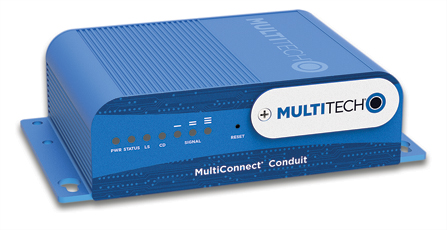
\includegraphics[width=0.4\textwidth]{Figures/Protocols/LoRaWAN/multitech_conduit.jpg}
    \caption{Concentrateur LoRaWAN Multitech Conduit}
    \label{fig-multitech_conduit}
\end{figure}

Les fournisseurs de réseaux doivent offrir un \textit{firmware} compatible avec les \textit{gateways}. Les \textit{firmwares} sont tous basés sur un code fournit par Semtech, nommé \texttt{Lora network packet forwarder}\footnote{\url{https://github.com/Lora-net/packet_forwarder}}. Comme son nom l'indique, ce code a pour but de transférer les données LoRa reçues vers un serveur avec un protocole d'échange spécifique. Le serveur répond ensuite à la \textit{gateway} en fonction de l'action qui doit être effectuée sur le périphérique, par exemple, lorsqu'un objet est autorisé à rejoindre le réseau après une procédure de \texttt{Join}.

\subsubsection{\textit{Network Server}}

Le \textit{Network} \textit{Serveur} est le gestionnaire du réseau. Il s'occupe de tous les paquets reçus sur le port 0. Les données reçues sur les autres ports sont transférées à la couche applicative gérée par l'\textit{Application Server}. Les différentes tâches incombant au \textit{Network Server} sont les suivantes \cite{ttnvideos_network:online} : 
\begin{itemize}
    \item Identification du périphérique qui souhaite communiquer avec le réseau. Les \textit{gateways} redirigent tous les paquets, ceux-ci doivent ensuite être triés \cite{ttnvideos_network:online};
    \item Contrôler le \textit{data rate} si le mode ADR (Adaptative Data Rate) est actif sur le périphérique;
    
    \item Configurer les paramètres radio ainsi que les différents timings des fenêtres de réceptions \cite{ttnvideos_network:online};
    
    \item Gestion des commandes de type MAC\footnote{\url{http://www.rfwireless-world.com/Tutorials/LoRaWAN-MAC-layer-inside.html}} \cite{HomeTheT94:online};
    
    \item Prévenir les attaques de type \textit{replay} en analysant les \textit{frame counters} des paquets;
    
    \item Gestion d'une queue de messages \textit{downlink} qui seront envoyés aux périphériques lors de la réception du prochain message \textit{uplink};
    
    \item Lors de l'envoi d'un message \textit{downlink}, le \textit{Network Server} s'occupe de la sélection de la \textit{gateway} qui doit envoyer le message. Celle-ci est sélectionnée en fonction du RSSI et du SNR vis-à-vis du périphérique sur le message \textit{uplink} reçu \cite{ttnvideos_network:online};
    
    \item Il s'occupe de la gestion du \textit{duty cycle} des \textit{gateways} afin de respecter les normes ETSI \cite{ttnvideos_network:online};
    
    \item Évite les conflits lors de l'envoi de messages \textit{downlink} sur une \textit{gateway}. Une \textit{gateway} ne peut envoyer qu'un seul message à la fois \cite{ttnvideos_network:online}.
\end{itemize}


Cette partie de l'architecture est traitée plus en détail en \cref{sec-stateoftheart_smartcanton}, via la présentation du projet SmartCanton.

\subsubsection{Join Server}

Le \textit{Join Server} n'est pas illustré sur la \cref{fig-lorawan_archtecture}, bien qu'il soit une brique indispensable lors de l'utilisation du mode OTAA. Lors de la réception d'un message de type \textit{Join Request}, le \textit{Network Server} le transfère au \textit{Join Server}. 

Il existe deux modes en LoRaWAN pour rejoindre un réseau. Le premier mode se nomme \textit{Over-the-Air Activation} (OTAA). Dans le mode OTAA, seules l'\texttt{App Key} et l'adresse \texttt{Dev EUI} (comparable à l'adresse MAC d'un périphérique) doivent être connues sur le périphérique. Le \texttt{Join Server} vérifie si le périphérique a été préalablement enregistré dans une base de données contenant une \texttt{App Key}, un \texttt{App EUI} (optionnel selon les cas), ainsi qu'un \texttt{Dev EUI}. Si tel est le cas, un \texttt{Join Accept} est retourné au périphérique qu'il a été accepté sur le réseau. Avec ce \textit{Join Accept}, il reçoit son \texttt{Dev Address} qui lui permet d'émettre sur le réseau avec cette adresse, ainsi les éléments nécessaires à la \texttt{Network Session Key} et \texttt{App Session Key} pour la communication. La procédure du \texttt{join} du mode OTAA est observée en détail en \cref{sec-security_lorawan} de ce document.

L'autre mode est \textit{Activation by Personalization} (ABP). Dans ce mode, toutes les informations nécessaires doivent être prodiguées manuellement au périphérique. Il faut donc spécifier le \textit{Device EUI} (normalement fixé par le fabricant), l'\textit{Application EUI}, le \textit{Device Address}, la \textit{Network Session Key}, ainsi que l’\textit{App Session Key}.

Le mode OTAA est préféré au mode ABP, non seulement parce qu'il simplifie l'ajout d'un périphérique au réseau, mais également parce qu'il ajoute un aspect de sécurité (cf. \cref{sec-security_lorawan}).

\subsubsection{Applications Server}


Le serveur d'application reçoit tous les paquets qui n'ont pas été envoyés sur le port 0. Toutes les \textit{payload} sont déchiffrées par ce serveur. Les données sont ensuite mises à disposition de l'utilisateur. Certains fournisseurs de réseau proposent des interfaces Web complètes pour visualiser les données décodées avec la \textit{App Session Key}. Ils offrent également la possibilité de rediriger ces données vers des fournisseurs d'application, par exemple Cayenne de MyDevices, qui accélèrent les prototypages rapides d'applications. Certains fournisseurs sont plus minimalistes et n'offrent qu'une interface de récolte de données à l'aide d'API diverses et variées. 

L'application finale est quant à elle entièrement libre pour l'utilisateur, la seule contrainte étant l'interface de communication proposée par le fournisseur de réseau. Chaque fournisseur peut proposer l'interface qu'il désire. Par exemple, TTN propose une interface basée sur un flux MQTT\footnote{\url{http://mqtt.org/}} et développe actuellement une interface AMQP\footnote{\url{https://www.amqp.org/}}. 


\subsection{\textit{Spreading Factor} et \textit{Data Rate}}
\label{sec-protocols_lorawan_spreading_factor}
%https://docs.exploratory.engineering/lora/dr_sf/


\begin{figure}[ht!]
    \centering
    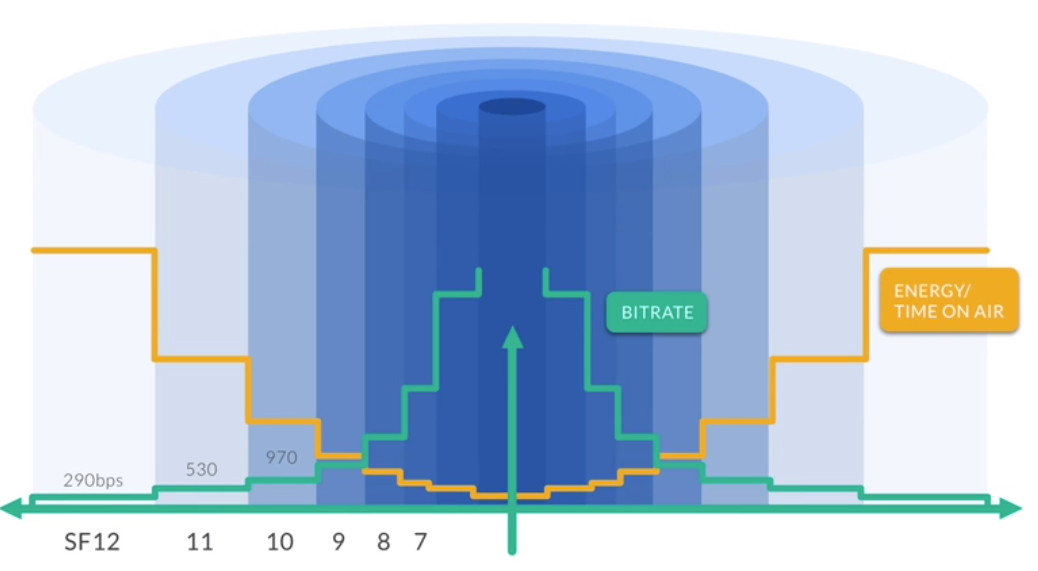
\includegraphics[width=0.7\textwidth]{Figures/Protocols/LoRaWAN/lora_datarate_airtime.png}
    \caption{Comparatif du temps d'émission d'une trame LoRaWAN en fonction de ses paramètres}
    \label{fig-lora_datarate_airtime}
\end{figure}

Le \textit{Spreading Factor} a d'ores et déjà été introduit en \cref{sec-stateoftheart_lora_spread_factor} lors de la présentation de la modulation LoRa. LoRaWAN utilise non seulement les SF pour l'émission, mais il ajoute également le concept de \textit{Data Rate} (DR). Le \cref{tab-datarate_eu} présente tous les \textit{data rate} qui sont autorisés en Europe \cite{Explorat95:online}. Chaque région possède des \textit{data rate} différents en fonction des législations. Chaque DR a une configuration différente en se basant sur un SF et sur la bande passante assignée. On constate en observant le \cref{tab-datarate_eu} que plus le DR est faible, plus le débit est faible. Avec un SF plus élevé, le temps d'émission est supérieur, ce qui a pour conséquence d'augmenter la portée en accentuant la sensibilité du récepteur. La taille du \textit{payload} est également affectée par le temps d'émission,et ce, afin d'éviter qu'on ne sature trop le réseau lors de l'émission avec un SF élevé. Une illustration plus visuelle de l'effet du DR est visible sur la \cref{fig-lora_datarate_airtime}.


\begin{table}[ht!]
\centering
\caption{Différents \textit{data rate} LoRaWAN avec leurs débits pour l'Europe}
\label{tab-datarate_eu}
\begin{tabular}{|l|l|r|r|}
\hline
\rowcolor[HTML]{BBDAFF} 
\multicolumn{1}{|c|}{\cellcolor[HTML]{BBDAFF}\textit{\textbf{Data Rate}}} & \multicolumn{1}{c|}{\cellcolor[HTML]{BBDAFF}\textbf{Configuration}} & \multicolumn{1}{c|}{\cellcolor[HTML]{BBDAFF}\textit{\textbf{bits/s}}} & \multicolumn{1}{c|}{\cellcolor[HTML]{BBDAFF}\textit{\textbf{Max payload}}} \\ \hline
DR0 & SF12/125kHz & 250 & 59 \\ \hline
DR1 & SF11/125kHz & 440 & 59 \\ \hline
DR2 & SF10/125kHz & 980 & 59 \\ \hline
DR3 & SF9/125kHz & 1 760 & 123 \\ \hline
DR4 & SF8/125kHz & 3 125 & 230 \\ \hline
DR5 & SF7/125kHz & 5 470 & 230 \\ \hline
DR6 & SF7/250kHz & 11 000 & 230 \\ \hline
DR7 & FSK: 50kbps & 50 000 & 230 \\ \hline
\end{tabular}
\end{table}


Pour éviter de fixer une valeur qui ne sera pas efficace dans toutes les situations, il est possible d'utiliser l'\textit{Adaptive Data Rate} (ADR) \cite{HomeTheT94:online}. L'ADR est un mécanisme qui a pour but d'optimiser les débits de données, le temps d'émission et, par conséquent, la consommation énergétique. L'ADR ne doit être utilisé que par des n\oe uds statiques. Ce sont les n\oe uds qui décident si cette option est activée ou non. Lorsque le réseau est informé de l'utilisation de l'ADR, celui-ci sauvegarde les 20 transmissions les plus récentes avec le \textit{frame counter}, \textit{signal-to-noise ratio} (SNR) et le nombre de \textit{gateways} qui ont reçu le paquet.

L'algorithme utilisé est décrit dans une \textit{application note} de Semtech, nommée \textit{Simple rate adaptation recommended algorithm}\footnote{\url{https://github.com/TheThingsNetwork/ttn/issues/265\#issuecomment-255092765}}.


\subsection{Paquets LoRaWAN}

\begin{figure}[ht!]
    \centering
    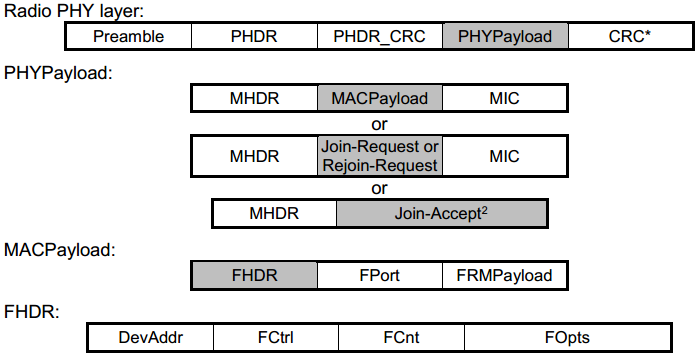
\includegraphics[width=0.9\textwidth]{Figures/Protocols/LoRaWAN/lorawan_mac_format_packets.png}
    \caption{Format des messages du protocole LoRaWAN}
    \label{fig-lorawan_mac_format_packets}
\end{figure}


Les paquets LoRaWAN se basent sur les paquets LoRa pour la transmission. Le squelette d'un paquet LoRa a d'ores et déjà été présenté en \cref{sec_stateOfTheArtLoRa}. Tous les paquets de données disposent d'une \texttt{PHY \textit{payload}} commençant par un octet de \textit{MAC header} (\texttt{MHDR}), suivi d'un \texttt{MAC \textit{payload}} (\texttt{MACPayload}). Le champ \texttt{PHYPayload} contient toute l'implémentation du protocole LoRaWAN. L'encapsulation des paquets au fil des différentes couches est visible sur la \cref{fig-lorawan_mac_format_packets}.


\begin{table}[ht!]
\centering
\caption{Différents champs contenus dans un MHDR}
\label{tab-header_MHDR_content}
\begin{tabular}{
>{\columncolor[HTML]{BBDAFF}}l |l|l|l|}
\cline{2-4}
\textbf{\textit{Bit\#}} & 7..5 & 4..2 & 1..0 \\ \hline
\textbf{\textit{MHDR bits}} & MType & RFU & Major \\ \cline{2-4} 
\end{tabular}
\end{table}

\begin{table}[ht!]
\centering
\caption{Différents types de messages MAC possibles}
\label{tab-mac_message_types}
\begin{tabular}{|l|l|}
\hline
\rowcolor[HTML]{BBDAFF} 
\multicolumn{1}{|c|}{\cellcolor[HTML]{BBDAFF}\textbf{\textit{MType}}} & \multicolumn{1}{c|}{\cellcolor[HTML]{BBDAFF}\textbf{\textit{Description}}} \\ \hline
000 & Join-request \\ \hline
001 & Join-accept \\ \hline
010 & Unconfirmed Data Up \\ \hline
011 & Unconfirmed Data Down \\ \hline
100 & Confirmed Data Up \\ \hline
101 & Confirmed Data Down \\ \hline
110 & Rejoin-request \\ \hline
111 & Proprietary \\ \hline
\end{tabular}
\end{table}

Les payload peuvent contenir différents types de paquets, ceux-ci étant définis dans l'entête MHDR dont les champs sont visibles sur la \cref{tab-header_MHDR_content}. Le type de message est codé sur 3 bits dans un champ nommé \texttt{MType}. LoRaWAN implémente 8 types de paquets visibles sur le \cref{tab-mac_message_types}. Les messages envoyés par les périphériques sont de types \texttt{Data UP}. Ceux-ci peuvent être confirmés ou non selon le type d'utilisation désirée. Le champ RFU signifie \textit{Reserved for Future Use} et le champ Major est utilisé pour spécifier la version de la spécification LoRaWAN utilisée (1.0 ou 1.1 actuellement).

La description complète des paquets est disponible dans le chapitre \texttt{MAC Message Formats} du document \texttt{LoRaWAN 1.1 Specification}\footnote{\url{https://www.lora-alliance.org/lorawan-for-developers}} de la LoRa Alliance. 


\subsection{Clés de chiffrement}

\begin{figure}[ht!]
    \centering
    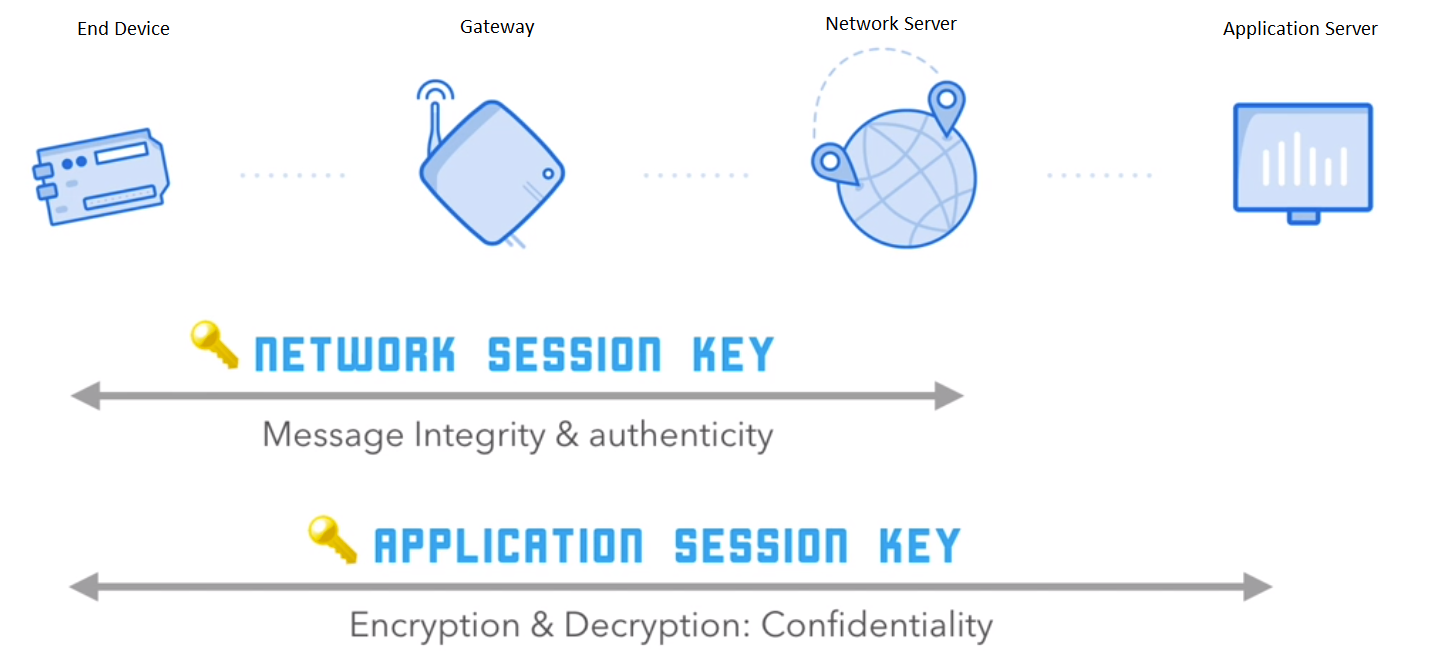
\includegraphics[width=0.8\textwidth]{Figures/Protocols/LoRaWAN/keys_explained.PNG}
    \caption{Rôles de la \textit{Network Session Key} et \textit{Application Session Key}}
    \label{fig-keys_explained}
\end{figure}

En OTAA, lorsqu'un périphérique souhaite rejoindre un réseau il ne dispose que d'une seule et unique clé, nommée AppKey. Une fois le réseau LoRaWAN rejoint, deux autres clés sont créées. L'aspect sécurité de ces clés, ainsi que la génération de celles-ci est vue plus en détail en \cref{sec-security_lorawan} de ce document. Pour l'heure, voici une liste des trois clés indispensables et leurs rôles respectifs : 
\begin{enumerate}
    \item \texttt{App Key} : doit être connue par le \textit{Join Server} et par le périphérique. C'est un secret partagé qui doit être bien gardé, puisque toutes les clés sont générées grâce à lui.
    \item \texttt{Network Session Key} : clé utilisée pour chiffrer les communications entre le périphérique et le \textit{Network Server}. Cette clé est générée à l'aide de l'App Key.
    \item \texttt{Application Session Key} : clé utilisée pour chiffrer les communications entre le périhpréqiue et l'\textit{Application Server}. Elle est également générée à l'aide de l'App Key.
\end{enumerate}

Sur la \cref{fig-keys_explained}, on peut visualiser l'utilisation des clés en fonction des types de messages envoyés.


% \subsection{Rejoindre un réseau LoRaWAN}


% Il existe deux modes en LoRaWAN pour rejoindre un réseau. Le premier est le mode \textit{Over-the-Air Activation} (OTAA). Dans le mode OTAA, la seule qui doit être connue sur le périphérique est la \texttt{App Key} ainsi que l'adresse \texttt{Dev EUI}. Le \texttt{Join Server} vérifie si le périphérique a été préalablement enregistré dans une base de données contenant une \texttt{App Key}, une \textit{App EUI} (optionnelle selon les cas) ainsi qu'une \texttt{Dev EUI}. Si c'est bien le cas, un \texttt{Join Accept} est retourné au périphérique lui indiquant qu'il a été accepté sur le réseau. Avec ce \textit{Join Accept}, il reçoit son \texttt{Dev Address} afin de pouvoir émettre sur le réseau au moyen de cette adresse. Il reçoit également les élément pour générer sa \texttt{Network Session Key} et \texttt{App Session Key} pour communication. La procédure du \texttt{join} du mode OTAA est détaillée en profondeur en \cref{sec-security_lorawan} de ce document.

% Le second mode se nomme \textit{Activation by Personalization} (ABP). Dans ce mode, toutes les informations nécessaires doivent être prodiguées manuellement au périphérique. Il faut donc spécifier le \textit{Device EUI} (normalement fixé par le fabricant), l'\textit{Application EUI}, la \textit{Device Address}, la \textit{Network Session Key}, ainsi que la \textit{App Session Key}.

% Le mode OTAA est préféré au mode ABP, non seulement parce qu'il simplifie l'ajout d'un périphérique au réseau, mais également parce qu'il ajoute un aspect de sécurité (cf. \cref{sec-security_lorawan}).





\subsection{Canaux d'émission}

La spécification LoRaWAN définit 3 canaux communs de 125 kHz pour la bande des 868 MHz (868.10, 868.30 et 868.50 MHz)\cite{HomeTheT94:online}. Ces canaux doivent être obligatoirement supportés par tous les réseaux LoRaWAN et par tous les périphériques. Ces 3 canaux sont ceux utilisés par tous les périphériques pour rejoindre un canal. Pendant la procédure de \texttt{Join}, le réseau peut demander aux périphériques d'ajouter de nouveaux canaux à sa liste. Ces canaux sont utilisés en \texttt{downlink}, mais également en \texttt{uplink}\cite{HomeTheT94:online}.



\subsection{Temps d'émission et nombre de paquets}

Le \textit{duty cycle} d'émission a été abordé en \cref{sec-stateoftheart_lora_dutycycle}. Les pourcentages d'utilisation des bandes de fréquences limitent les utilisations qui peuvent être faites de ce protocole. Le temps d'émission est affecté par les paramètres choisis pour l'émission. Comme expliqué en \cref{sec-stateoftheart_lora_spread_factor} et en \cref{sec-protocols_lorawan_spreading_factor}, le \textit{spreading factor} et le \textit{coding rate} augmentent considérablement le temps d'émission. 


Outre ces restrictions, certains fournisseurs de réseau limitent encore plus drastiquement l'utilisation de la bande de fréquence. Par exemple, \textit{The Things Network} (TTN) applique une \textit{Fair Access Policy} \footnote{\url{https://www.thethingsnetwork.org/forum/t/limitations-data-rate-packet-size-30-seconds-uplink-and-10-messages-downlink-per-day-fair-access-policy/1300}} afin de réduire la charge d'accès sur leur réseau \cite{Limitati95:online}. Les types de limitations sont les suivantes : 
\begin{enumerate}
    \item Une moyenne de 30 secondes en émission \textit{uplink}, par jour et par périphérique;
    \item Maximum 10 \textit{downlink} messages par jour, en incluant des confirmations pour les messages de type \textit{confirmed uplink};
    \item Les périphériques avec un SF de 11 ou 12 \textbf{fixe} ne sont pas autorisés à rejoindre le réseau (ceci ne s'applique pas aux périphériques avec l'ADR activé).
\end{enumerate}

La limitation de 30 secondes d'émission est la plus restrictive. Par exemple, si un périphérique envoi un \textit{payload} de 55 bytes en utilisant le \textit{data rate} le plus élevé, cela crée une émission de 71.81 millisecondes\cite{Limitati95:online}. En respectant uniquement les standards européens, ceci signifie qu'un périphérique doit attendre 71,09 secondes avant de pouvoir envoyer une nouvelle trame. Cependant, avec la limitation supplémentaire de TTN, le périphérique ne peut envoyer que 417 paquets de 71.81 par jours; ce qui signifie en moyenne un paquet toutes les 207 secondes ainsi en appliquant ces limitations, une \textit{gateway} TTN peut avoir jusqu'à 1000 n\oe uds connectés \cite{Limitati95:online}. TTN propose un tableau sur Google Sheet\footnote{\url{https://docs.google.com/spreadsheets/d/1QvcKsGeTTPpr9icj4XkKXq4r2zTc2j0gsHLrnplzM3I}} éditable pour calculer le nombre de paquets possibles sur le réseau en fonction de la configuration appliquée sur le périphérique.

\subsection{Spécification LoRaWAN 1.1}
\label{sec-protocols_lorawan_spec_1_1}

La LoRa Alliance a finalisé la spécification V1.1 en octobre 2017\footnote{\url{https://www.lora-alliance.org/lorawan-for-developers}}. Il faut à présent du temps pour qu'elle se démocratise sur les différents périphériques. Actuellement, le CMWX1ZZABZ ne propose pas de \textit{firmware} pour le support de cette spécification. Celle-ci ne nécessite par ailleurs pas de nouveau matériel, son implémentation étant entièrement logicielle. Certaines nouveautés sur la sécurité sont exposées en \cref{sec-security_lorawan_1_1}. 

\begin{figure}[ht!]
    \centering
    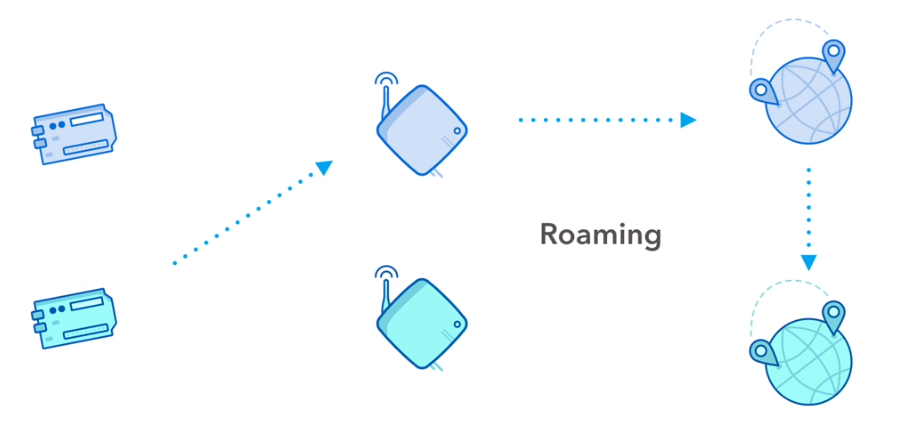
\includegraphics[width=0.6\textwidth]{Figures/Protocols/LoRaWAN/lorawan_roaming.png}
    \caption{Roaming LoRaWAN}
    \label{fig-lorawan_roaming}
\end{figure}

LoRaWAN 1.1 ajoute le support du \textit{roaming} entre différents opérateurs. Le concept est visible sur la \cref{fig-lorawan_roaming}, où l'on peut voir un périphérique transmettant un paquet capturé par une \textit{gateway} d'un réseau auquel il n'appartient pas. Si le \textit{Network Server} ne reconnait pas le périphérique comme appartenant à son réseau, il \textit{forward} les paquets vers le \textit{Network Server} de l'opérateur d'origine. Le principe général est identique au \textit{roaming} appliqué à la téléphonie mobile.

